%%%%%%%%%%%%%%%%%%%%%%%%%%%%%%%%%%%%%%%%%
% Journal Article
% LaTeX Template
% Version 1.3 (9/9/13)
%
% This template has been downloaded from:
% http://www.LaTeXTemplates.com
% http://en.wikibooks.org/wiki/LaTeX/Mathematics
% Original author:
% Frits Wenneker (http://www.howtotex.com)
%
% License:
% CC BY-NC-SA 3.0 (http://creativecommons.org/licenses/by-nc-sa/3.0/)
%
%%%%%%%%%%%%%%%%%%%%%%%%%%%%%%%%%%%%%%%%%

%----------------------------------------------------------------------------------------
%	PACKAGES AND OTHER DOCUMENT CONFIGURATIONS
%----------------------------------------------------------------------------------------

%\documentclass[twoside]{article}
\documentclass[a4paper,12pt]{article}

%\usepackage{lipsum} % Package to generate dummy text throughout this template
\usepackage{mathtools} % package fixes some amsmath quirks and adds some useful settings, symbols, and environments to amsmath
\usepackage[sc]{mathpazo} % Use the Palatino font
\usepackage[T1]{fontenc} % Use 8-bit encoding that has 256 glyphs
\linespread{1.05} % Line spacing - Palatino needs more space between lines
\usepackage{microtype} % Slightly tweak font spacing for aesthetics

\usepackage[hmarginratio=1:1,top=32mm,columnsep=20pt]{geometry} % Document margins
\usepackage{multicol} % Used for the two-column layout of the document
\usepackage[hang, small,labelfont=bf,up,textfont=it,up]{caption} % Custom captions under/above floats in tables or figures
\usepackage{booktabs} % Horizontal rules in tables
\usepackage{float} % Required for tables and figures in the multi-column environment - they need to be placed in specific locations with the [H] (e.g. \begin{table}[H])
\usepackage{hyperref} % For hyperlinks in the PDF

\usepackage{lettrine} % The lettrine is the first enlarged letter at the beginning of the text
\usepackage{paralist} % Used for the compactitem environment which makes bullet points with less space between them

\usepackage{cite}
%\usepackage[numbers,sort&compress]{natbib}
%\usepackage[style=numeric]{biblatex}
%\addbibresource{thomastsai.bib}
%\bibliographystyle{ieeetr}

\usepackage{abstract} % Allows abstract customization
\renewcommand{\abstractnamefont}{\normalfont\bfseries} % Set the "Abstract" text to bold
\renewcommand{\abstracttextfont}{\normalfont\small\itshape} % Set the abstract itself to small italic text

%http://en.wikibooks.org/wiki/LaTeX/Floats,_Figures_and_Captions
\usepackage{graphicx}
\usepackage{subcaption}
\graphicspath{ {dft/} }
\DeclareGraphicsExtensions{.pdf,.png,.jpg}

\usepackage{fancyhdr} % Headers and footers
\pagestyle{fancy} % All pages have headers and footers
\fancyhead{} % Blank out the default header
\fancyfoot{} % Blank out the default footer
%\fancyhead[C]{Running title $\bullet$ October 2014 $\bullet$ Vol. XXI, No. 1} % Custom header text
%\fancyfoot[RO,LE]{\thepage} % Custom footer text

\usepackage{pgfplots}
\pgfplotsset{compat=newest}

%\usepackage{titlesec} % Allows customization of titles
%\renewcommand\thesection{\Roman{section}} % Roman numerals for the sections
%\renewcommand\thesubsection{\Roman{subsection}} % Roman numerals for subsections
%\titleformat{\section}[block]{\large\scshape\centering}{\thesection.}{1em}{} % Change the look of the section titles
%\titleformat{\subsection}[block]{\large}{\thesubsection.}{1em}{} % Change the look of the section titles

\newtheorem{theorem}{Theorem}

%----------------------------------------------------------------------------------------
%	TITLE SECTION
%----------------------------------------------------------------------------------------

\title{\vspace{-15mm}\fontsize{24pt}{10pt}\selectfont\textbf{Study Report: Object Detection with Pixel Intensity Comparisons Organized in Decision Trees}} % Article title

\author{
\large
\textsc{Thomas Tsai}\thanks{Thomas Tsai is a RD VP in biotrump inc.}\\[2mm] % Your name
\normalsize www.biotrump.com \\ % Your institution
\normalsize \href{mailto:thomas@biotrump.com}{thomas@biotrump.com} % Your email address
\vspace{-5mm}
}
\date{}

%----------------------------------------------------------------------------------------

\begin{document}

\maketitle % Insert title

%----------------------------------------------------------------------------------------
%	ABSTRACT
%----------------------------------------------------------------------------------------

\begin{abstract}

%\noindent \lipsum[1] % Dummy abstract text
Normalized Pixel Difference (\textbf{NPD}) feature is computed as the difference 
to sum ratio between two pixel values, inspired by the \textbf{Weber Fraction} in
experimental psychology. \textbf{NPD} is \textbf{scale invariant, bounded}, 
and is able to \textbf{reconstruct} the original image. \textbf{Second}, we learn 
the optimal subset of NPD features and their combinations via \textbf{regression trees}, 
so that \textbf{complex face manifolds can be partitioned by the learned rules}. 
Only a single cascade classifier is needed to handle unconstrained face detection.
Furthermore, we show that the NPD features can be efficiently obtained from a \textbf{look up table}, 
and the detection template can be easily scaled, making the proposed face detector very fast 
(about \textbf{178 FPS for 640x480} resolution videos and \textbf{30 FPS for 1920x1080} 
resolution videos on a desktop PC, about \textbf{6 times} faster than OpenCV). 
Experimental results on \textbf{three public face} datasets (\textbf{FDDB, GENKI, and CMU-MIT}) 
show that the proposed method outperforms the state-of-the-art methods in detecting unconstrained 
faces with \textbf{arbitrary pose variations} and \textbf{occlusions} in cluttered scenes.
\cite{DBLP:journals/corr/LiaoJL14}
\end{abstract}

%----------------------------------------------------------------------------------------
%	ARTICLE CONTENTS
%----------------------------------------------------------------------------------------

%\begin{multicols}{2} % Two-column layout throughout the main article text
%\end{multicols}

%\onecolumn

\section{Introduction}
The objective of face detection is to find and locate faces in an image. It is the first step in automatic face
recognition applications. Face detection has been well studied for frontal and near frontal faces.


The \textbf{Viola and Jones} face detector \cite{Viola2001Rapid} is the most well 
known face detection algorithm, which is based on \textbf{Haar-like} features and 
\textbf{cascade AdaBoost classifier}\cite{Friedman98additivelogistic}. However, 
in unconstrained scenes such as \textbf{faces in a crowd}, state-of-the-art face 
detectors fail to perform well due to \textbf{large pose variations, illumination variations, occlusions, expression variations, out-of-focus blur, and low image resolution}.\\

Numerous face detection methods have been developed following Viola and Jones work \cite{Viola2001Rapid}, 
mainly focusing on extracting \textbf{different types of features} and developing \textbf{different cascade structures}. 
A variety of complex features have been proposed to \textbf{replace the Haar-like} features used in \cite{Viola2001Rapid}. 
While these methods can improve the face detection performance to some extent,
they generate a \textbf{very large number} (hundreds of thousands) of features and the resulting systems take
\textbf{too much time to train}.\\

Another development in face detection has been to learn \textbf{different cascade structures for multiview face detection}, 
such as \textbf{parallel cascade} \cite{conf/fgr/WuAHL04}, \textbf{pyramid architecture}\cite{journals/pami/LiZ04}, 
and \textbf{Width-First-Search (WFS) tree} \cite{huang_et_al_2007}. All these methods need to learn 
\textbf{one cascade classifier for each specific facial view (or view range)}. In unconstrained scenarios, 
however, it is \textbf{not easy} to define all possible views of a face, and the \textbf{computational cost increases} 
with an increasing number of classifiers in complex cascade structure. Moreover, these approaches \textbf{require manual labeling} 
of face pose in each training image. While some of the available methods 
\cite{conf/fgr/WuAHL04}, \cite{Viola2001Rapid}, \cite{huang_et_al_2007}, can  \textbf{handle multiview faces}, 
they are \textbf{not able to} simultaneously consider other challenges such as  \textbf{occlusion}.\\

In fact, since these methods require  \textbf{partitioning multiview data into known poses}, 
occlusion is not easy to handle in this way. On the other hand, while several studies addressed face detection under occlusion, 
they constrained themselves to detect only frontal faces under occlusion.\\

A robust face detection algorithm should be effective under \textbf{arbitrary variations in pose and occlusion, 
which remains an unresolved challenging problem}. \\

\textbf{First}, a simple pixel-level feature, called the \textbf{Normalized Pixel Difference (NPD)}. 
An NPD is computed as the ratio of the difference between any two pixel intensity values to the sum of their values, in the
same form as the Weber Fraction in experimental psychology [23]. The NPD feature has \textbf{several desirable properties}, 
such as scale invariance, boundedness, and ability to reconstruct the original image. 
we further show that NPD features can be obtained from a look up table, and the resulting face detection template 
can be easily scaled for multiscale face detection. \\

\textbf{Secondly}, we develop a method to construct a \textbf{single cascade AdaBoost classifier} that can effectively deal  
with \textbf{complex face manifolds} and handle \textbf{arbitrary pose} and \textbf{occlusion} conditions. 
While the individual NPD feature may have \textbf{weak discriminative ability}, 
a \textbf{subset of NPD features} can be \textbf{optimally learned} and 
\textbf{combined to construct} more discriminative features in a \textbf{regression tree}. In this way, 
different types of faces can be \textbf{automatically divided} into different leaves of a regression tree, 
and the \textbf{complex face manifold} in high dimensional space can be partitioned in the learning process. \\

This is a \textbf{divide and conquer} strategy to tackle unconstrained face detection in a \textbf{single classifier}, 
without \textbf{pre-labeling of views} in the training set of face images. 
The resulting face detector is robust to \textbf{variations in pose, occlusion, and illumination}, 
as well as to \textbf{blur and low image} resolution. This work is summarized as follows:

\begin{compactitem}
\item A new type of feature, called NPD is proposed, which is efficient to compute and has several desirable properties, 
including scale invariance, boundedness, and enabling reconstruction of the original image.
\item A subset of NPD features is \textbf{automatically learned} and \textbf{combined} 
in regression trees to boost their discriminability. In this way, \textbf{only a single cascade AdaBoost classifier} 
is needed to handle unconstrained faces with occlusions and arbitrary viewpoints, 
without pose labeling or clustering in the training stage.\\
\end{compactitem}

The advantages of the proposed approach include:
\begin{compactitem}
\item The NPD feature evaluation is extremely fast, requiring a single memory access using a \textbf{look up table}.
\item \textbf{Multiscale} face detection can be easily achieved by applying pre-scaled detection templates.
\item The unconstrained face detector does not depend on pose specific cascade structure design; 
pose labeling or clustering in the training stage is also not required.
\item The face detector is able to handle \textbf{illumination variations, pose variations, occlusions, 
outof-focus blur, and low resolution} face images in unconstrained scenarios.
\end{compactitem}


\section{NORMALIZED PIXEL DIFFERENCE FEATURE SPACE}
\begin{figure}
\centering
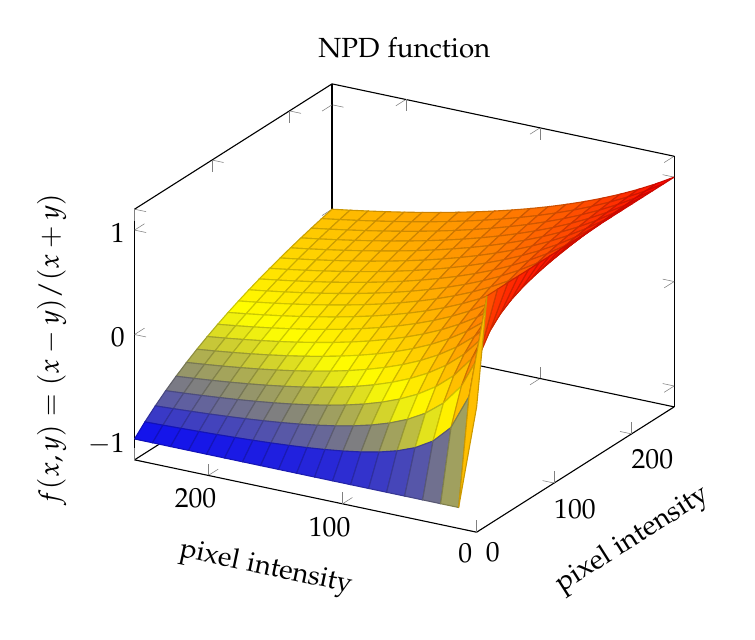
\begin{tikzpicture}
	\begin{axis}[
	title={NPD function},
	view/h=-30,
	view/az=-60,
	xlabel=pixel intensity,
	ylabel=pixel intensity,
	zlabel={$f(x,y)=(x-y)/(x+y)$},
	xlabel style={sloped like x axis},
	ylabel style={sloped}
	]
	\addplot3[surf,shader=faceted,
		samples=20,domain=0:255] 
		{(x-y)/(x+y)};
	\label{pgfplots:NPD}
	\end{axis}
\end{tikzpicture}
	\caption{NPD}
	\label{fig:npd}
\end{figure}

The Normalized Pixel Difference (NPD) feature between
two pixels in an image is defined as

\begin{equation}
\label{eq:NPD}
f(x,y)=
\begin{cases}
    0,					& if \ x=0,y = 0\\
    \frac{x-y}{x+y},   & \text{x} \ge 0\ and\ y \ge 0
\end{cases}
\end{equation}

where x and y $\ge$ 0 are \textbf{intensity} values of the two pixels. 
The NPD feature measures the relative difference between two pixel values. 
The sign of $f(x, y)$ indicates the \textbf{ordinal relationship} between the two pixels x and y , 
and the \textbf{magnitude} of $f(x, y)$ measures the relative difference (as a percentage of the 
joint intensity x+y) between x and y. The definition \textbf{f(0, 0) = 0} is reasonable because 
there is \textbf{no difference} between the two pixels x and y. And f(x,x)=0 along the x=y.\\

Weber, a pioneer in experimental psychology, stated that the \textbf{just-noticeable difference in the magnitude
change of a stimulus is proportional to the magnitude of the stimulus, rather than its absolute value.
This is known as the Weber\'s Law}. In other words, the human perception of difference in stimulus is often
measured as a fraction of the original stimulus, that is, in a form \textbf{$\Delta$I/I}, which is called 
the \textbf{Weber Fraction}.\\

Chen et al. [43] proposed a local image descriptor, called Weber\'s Law Descriptor for face recognition,
which was computed from Weber Fractions of pixels in a 3 x 3 window. The proposed feature in \eqref{eq:NPD}
has also been used in other fields such as remote sensing, where the Normalized Difference Vegetation
Index (NDVI) [44] is defined as the difference to sum ratio between the visible red and the near infrared
spectra to estimate the green vegetation coverage.\\


The NPD feature has a number of \textbf{desirable properties}:
\begin{compactitem}
\item \textbf{First}, the NPD feature is \textbf{antisymmetric}, so either f(x, y) or f(y, x) is acceptable for feature representation, resulting in a reduced feature space. 
Therefore, in an \textbf{s x s} image patch (vectorized as \textbf{p x 1}, where \textbf{p = s $\cdot$ s)}, 
NPD feature \textbf{$f(x_i, x_j)$} for pixel pairs($x_i,x_j$),\textbf{ 1 $\le$ i < j $\le$ p} is computed, 
resulting in \textbf{d=p(p-1)/2} features, combination C$\binom{p}{2}$. 
For example, in a 20x20 face template, there are d=C$\binom{20x20}{2}$= (20x20)x(20x20-1)/2 = 79800 NPD features
in total. We call the resulting feature space the \textbf{NPD feature space, denoted as $\Omega_{npd}  (\in R_d)$}.\\

\item \textbf{Second}, the \textbf{sign of f(x,y)} is an indicator of the \textbf{ordinal relationship} between x and y. 
Ordinal relationship has been shown to be an effective encoding for object detection and recognition [25], [26], [28] 
because ordinal relationship encodes the intrinsic structure of an object image and it is \textbf{invariant under various illumination changes} [25].
However, simply using the sign to encode the ordinal relationship is likely to be \textbf{sensitive to noise} when x and y have similar values. 
In the next section we will show how to learn robust ordinal relationships with NPD features.\\

\item \textbf{Third}, the NPD feature is \textbf{scale invariant}, which is expected to be robust against
\textbf{illumination changes}. This is important for image representation, since illumination change is always a troublesome issue for
both object detection and recognition.\\

\item \textbf{Fourth}, as shown in Appendix A, the NPD feature f(x,y) is \textbf{bounded in [-1,1]}. 
The bounded property makes the NPD feature amenable to histogram binning or threshold learning in tree-based classifiers [1]. 
Fig. 2 shows that f(x, y) is a bounded function and it defines a nonlinear surface.

\begin{theorem}
\label{Reconstruction}
(Reconstruction): Given the NPD feature vector 
\\$f = (f(x_1, x_2), f(x_1, x_3), . . . ,f(x_{p-1}, x_p))^T$ $\in \Omega_{npd}$ , the original image intensity values $I = (x_1, x_2, . . . , x_p)^T$ can be reconstructed up to a scale factor.
\end{theorem}

The proof of theorem \ref{Reconstruction} is shown in Appendix B, which also gives a linear-time approach to reconstruct
the original image up to a scale factor. theorem \ref{Reconstruction} states that each point in the feature 
space $\Omega_{npd}$ corresponds to a group of intensity-scaled images in the original pixel intensity space. 
In contrast, the scale invariance property says that all intensity-scaled images are ''compressed'' to a point
in the bounded feature space $\Omega_{npd}  (\in R_d)$. Therefore, $\Omega_{npd}  (\in R_d)$ is a feature
space which is invariant to scale variations, but it carries all the necessary information from the original space.
\end{compactitem}

\section{Pair-Wise Ordinal Relationship}

\begin{figure}[h!]
  \centering
  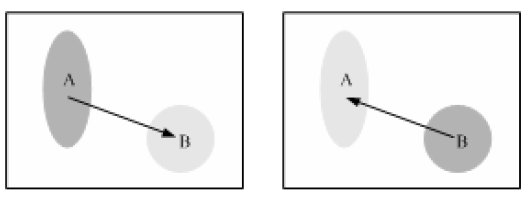
\includegraphics[width=\textwidth, keepaspectratio=true]{pair-wise-ordinal.jpg}
  \caption{Ordinal measure of relationship between two regions. 
  An arrow points from the darker region to the brighter one. Left: Region A is darker than B}
 \label{fig:pair-wise-ordinal}
\end{figure}

We could easily rank or order the heights or weights of two persons, 
but it is hard to answer their precise differences. For computer vision, the absolute intensity
information associated with an face can vary because it can \textbf{changes under various illumination
settings}. However, ordinal relationships among neighborhood image pixels
or regions present some stability with such changes and reflect the intrinsic natures of the face.
An ordinal feature encodes an ordinal relationship between two concept. 
\autoref{fig:pair-wise-ordinal} gives an example in which the average intensities between regions A and B are compared
to give the \textbf{ordinal code of 1 or 0}. Ordinal features are efficient to compute. Moreover,
the information entropy of the measure is maximized because the ordinal code has
nearly equal probability of being 1 or 0 for arbitrary patterns. \cite{conf/icb/LiaoLZSLT06}

\begin{figure}[ht]
  \centering
  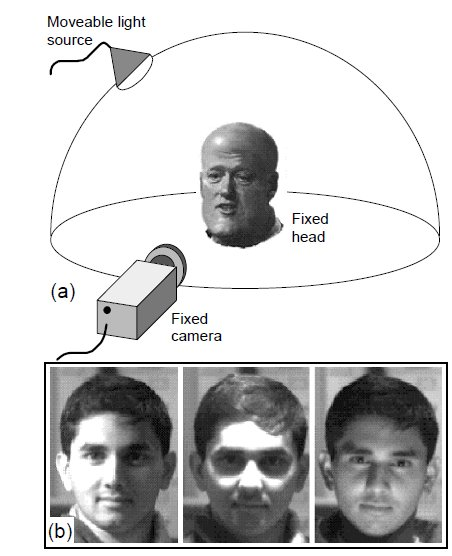
\includegraphics[width=0.95\textwidth, keepaspectratio=true]{various-illumination-setting.jpg}
  \caption{The absolute brightnesses and even their relative magnitudes change under 
  different lighting conditions but several pair-wise ordinal relationships are invariant. \cite{Sinha:2002:QRR:648248.751730}}
 \label{fig:various-illumination-setting}
\end{figure}

\autoref{fig:face-pair-wise-ordinal} shows several pairs of average brightness values over localized patches
for each of the three images included in \autoref{fig:various-illumination-setting}(b).
For instance, the average brightness of the left eye is always less than that of the forehead, 
irrespective of the lighting conditions. The relative magnitudes of the two brightness values may change, 
but the sign of the inequality does not. In other words, the ordinal relationship between the average
brightnesses of the <left-eye, forehead> pair is invariant under lighting changes.

\autoref{fig:face-pair-wise-ordinal} also shows several other such pair-wise invariances. 
By putting all of these pair-wise invariances together, we obtain a larger composite invariant 
(\autoref{fig:face-ratio-template}). We call this invariant a \textbf{'ratio template'}, 
given that it is comprised of a set of binarized ratios of image brightnesses. 
It is worth noting that dispensing with precise measurements of image brightnesses not only leads to immunity to illumination variations, but also renders the ratio-template robust in the face of sensor noise. 

The human visual system is far better at making relative brightness judgments than absolute ones. 
The ''ratio-template'' is \textbf{not a strict invariant}. There exist special cases where it breaks. 
One such situation arises when the face is strongly \textbf{illuminated from below}.
However, for almost all \textbf{''normal''} lighting conditions \textbf{(light sources at or above the level of the head)}, the ratio-template serves as a robust invariant. \cite{Sinha:2002:QRR:648248.751730}

\begin{figure}[ht]
  \centering
  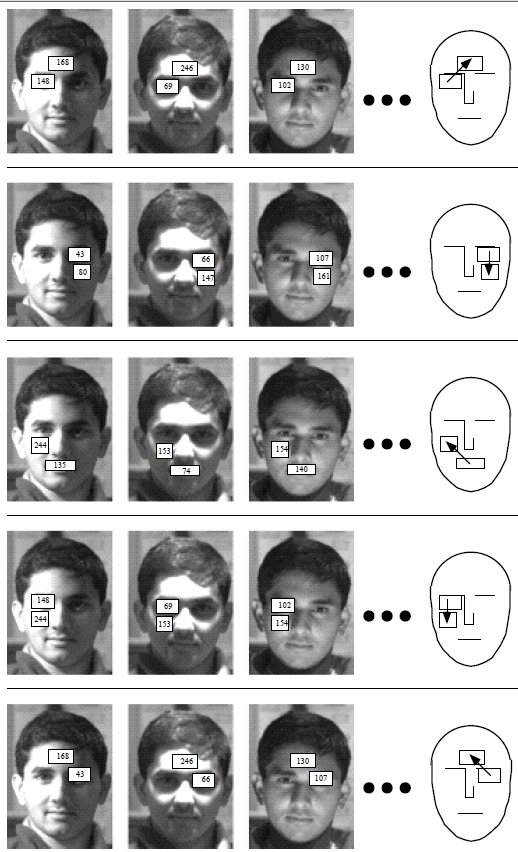
\includegraphics[width=0.95\textwidth, keepaspectratio=true]{face-pair-wise-ordinal.jpg}
  \caption{The absolute brightnesses and even their relative magnitudes change under 
  different lighting conditions but several pair-wise ordinal relationships are invariant. \cite{Sinha:2002:QRR:648248.751730}}
 \label{fig:face-pair-wise-ordinal}
\end{figure}

\begin{figure}[hb]
  \centering
  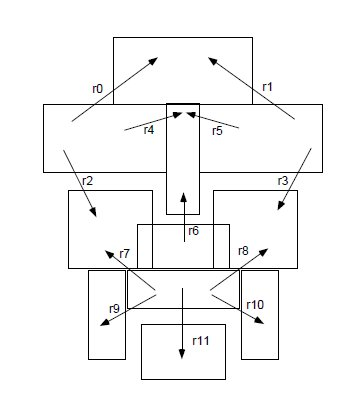
\includegraphics[width=\textwidth, keepaspectratio=true]{face-ratio-template.jpg}
  \caption{By putting together several pair-wise invariants, we obtain what we call a 
  ''ratio template''. This is a representation of the invariant ordinal structure of the 
  image brightness on a human face under widely varying illumination conditions.\cite{Sinha:2002:QRR:648248.751730}}
 \label{fig:face-ratio-template}
\end{figure}

%----------------------------------------------------------------------------------------
%	REFERENCE LIST
%----------------------------------------------------------------------------------------
\clearpage
%\printbibliography
%\bibliography{abbr_long,pubext}
% Note the bib files list should lack of whitespace between the commas and the next bib file.
\bibliography{nips14,thomastsai}
\bibliographystyle{ieeetr}

%\begin{thebibliography}{99} % Bibliography - this is intentionally simple in this template

%\bibitem[Figueredo and Wolf, 2009]{Figueredo:2009dg}
%Figueredo, A.~J. and Wolf, P. S.~A. (2009).
%\newblock Assortative pairing and life history strategy - a cross-cultural
%  study.
%\newblock {\em Human Nature}, 20:317--330.
 
%\end{thebibliography}

%----------------------------------------------------------------------------------------

%\end{multicols}
\end{document}
